% This file was created by tikzplotlib v0.8.5.
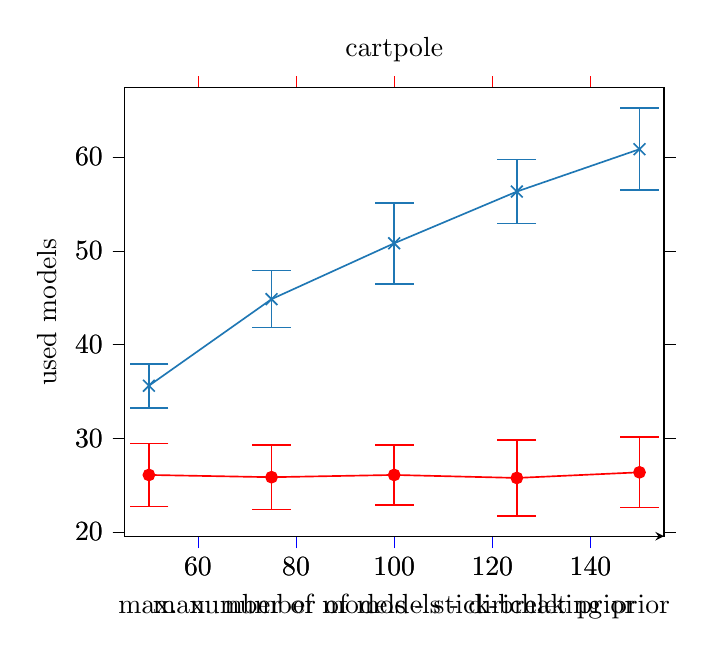
\begin{tikzpicture}

\definecolor{color0}{rgb}{0.12156862745098,0.466666666666667,0.705882352941177}

\begin{axis}[
tick align=outside,
tick pos=both,
title={cartpole},
x grid style={white!69.01960784313725!black},
xlabel={max. number of models - stick-breaking prior},
xmin=45, xmax=155,
xtick style={color=red},
y grid style={white!69.01960784313725!black},
ylabel={used models},
ymin=19.5428121928384, ymax=67.3843283188103,
ytick style={color=black}
]
\path [draw=red, semithick]
(axis cs:50,22.7104896498156)
--(axis cs:50,29.4495103501844);

\path [draw=red, semithick]
(axis cs:75,22.3795953993789)
--(axis cs:75,29.3004046006211);

\path [draw=red, semithick]
(axis cs:100,22.9061064920196)
--(axis cs:100,29.2538935079804);

\path [draw=red, semithick]
(axis cs:125,21.7174265622008)
--(axis cs:125,29.8025734377992);

\path [draw=red, semithick]
(axis cs:150,22.5982982574372)
--(axis cs:150,30.1217017425628);

\addplot [semithick, red, mark=-, mark size=7, mark options={solid}, only marks]
table {%
50 22.7104896498156
75 22.3795953993789
100 22.9061064920196
125 21.7174265622008
150 22.5982982574372
};
\addplot [semithick, red, mark=-, mark size=7, mark options={solid}, only marks]
table {%
50 29.4495103501844
75 29.3004046006211
100 29.2538935079804
125 29.8025734377992
150 30.1217017425628
};
\addplot [semithick, red, mark=*, mark size=2, mark options={solid}]
table {%
50 26.08
75 25.84
100 26.08
125 25.76
150 26.36
};
\end{axis}

\begin{axis}[
axis x line=top,
tick align=outside,
tick pos=both,
x grid style={white!69.01960784313725!black},
xlabel={max. number of models - dirichlet prior},
xmin=45, xmax=155,
xtick style={color=blue},
y grid style={white!69.01960784313725!black},
ymin=19.5428121928384, ymax=67.3843283188103,
ytick style={color=black}
]
\path [draw=color0, semithick]
(axis cs:50,33.2505319751059)
--(axis cs:50,37.9494680248941);

\path [draw=color0, semithick]
(axis cs:75,41.797895465307)
--(axis cs:75,47.882104534693);

\path [draw=color0, semithick]
(axis cs:100,46.4825933710154)
--(axis cs:100,55.1174066289846);

\path [draw=color0, semithick]
(axis cs:125,52.9056772267403)
--(axis cs:125,59.7343227732597);

\path [draw=color0, semithick]
(axis cs:150,56.4702860505521)
--(axis cs:150,65.209713949448);

\addplot [semithick, color0, mark=-, mark size=7, mark options={solid}, only marks]
table {%
50 33.2505319751059
75 41.797895465307
100 46.4825933710154
125 52.9056772267403
150 56.4702860505521
};
\addplot [semithick, color0, mark=-, mark size=7, mark options={solid}, only marks]
table {%
50 37.9494680248941
75 47.882104534693
100 55.1174066289846
125 59.7343227732597
150 65.209713949448
};
\addplot [semithick, color0, mark=x, mark size=3, mark options={solid}]
table {%
50 35.6
75 44.84
100 50.8
125 56.32
150 60.84
};
\end{axis}

\end{tikzpicture}
